\section{Law of motion of capital and debt}

This model is set within a partial equilibrium framework where firms are differentiated by their productivity levels.
They have the option to fund their operations by obtaining loans from financial intermediaries, as outlined by
\cite{bernanke1995inside}, or by retaining dividends. The capital at any time \(t\) is calculated by
adjusting capital from the previous period for depreciation (\(\delta\)), then adding gross investment (\(I\)), thus the
law of motion of capital stock is: 
\begin{align*}
    k_{t+1} &= k_{t}(1 - \delta)  + I_t  
\end{align*} 
We can rearrange  the above equation and get gross investment at time t
\begin{align}
    I_t &= k_{t+1} - k_{t}\left(1-\delta\right) \label{eq1}
\end{align} 
The \ref{eq1} equation states gross investment at time t is equal to the net capital formation plus replacement
of depreciated capital. 
The flow of funds constraint is:
\begin{align}
    I_t + R b_{t} + d_t &= f(k_t) + b_{t+1} \label{eq2}
\end{align}
where \(R\) denotes the gross interest rate and \(b_{t}\) represents the debt from period t.
The components of the flow of funds (f-of-f) at time \(t\) include:
\begin{enumerate}
    \item \(I_t\) gross investment at time t
    \item \(R b_{t}\) repayment of debts (principal and interest) 
    \item \(d_t\) dividends distributed at time t
\end{enumerate}

Conversely, the right-hand side details the sources of fund inflows:
\begin{enumerate}
    \item \(f(k_{t}) \) output at time t+1
    \item  \(b_t\) debt at time t+1
\end{enumerate}

The f-of-f constraint can be rewritten as the law of motion of debt: 
\begin{align} 
    b_{t+1} &= R b_{t} + I_{t} - S_{t}  \label{eq2'}
\end{align} 
where \(S_{t} = f(k_{t}) - d_t\) represents  retained earnings.
This formulation clarifies that the debt level at time \(t+1\) is the sum of the repayment for the previous period's debt
(both principal and interest) and the net investment, adjusted for internal financing.

From equations \ref{eq1}, \ref{eq2'} and the definition of net worth \(n_{t+1}=k_{t+1}-b_{t+1}\), we derive the law of motion for net worth as follows:
\begin{align*}
    n_{t+1}&=k_{t+1}-b_{t+1} = k_{t}(1-\delta) + I_t - R b_{t} - I_t + S_{t} \\
    &= k_{t} - \delta k_{t} - b_{t} - r b_{t}+ S_t \\
    &= n_{t} - \delta k_{t} - r b_{t} + \left[f\left({k_t}\right) - d_t \right]
\end{align*}

The net worth or equity of the firm is given by the net worth of the previous period less the depreciated capital, less
the interest matured from the previous period augmented by the retained earnings. Therefore a firm can increase its
net worth only through increasing the retained earnings levels, thus increasing output or decreasing dividends.
Using equations \ref{eq1} and \ref{eq2}, we get the flow of funds constraint for capital:
\begin{align}
    k_{t+1}=k_{t}(1-\delta)- R b_{t} - d_t + f(k_{t})+b_{t+1} \label{eq3}
\end{align}
The above equation describes how capital evolves: capital at time \(t+1\) is equal to capital at time t
net of depreciation, less the repayment of debt (principal + interest), augmented by retained earnings. 
\subsection{Steady State}

From \ref{eq1}, assuming (\(k_{t+1}=k_{t}=\widehat{k}\)), we get the steady state investment:
\begin{align}
    \widehat{k}&=\widehat{k}\left(1-\delta\right) + \widehat{I} \nonumber\\
    \widehat{I}&=\delta \widehat{k}  \label{eq4}
\end{align}
\ref{eq4} states that in the steady state, the firm will invest only to substitute depreciated capital(\(\delta
\widehat{k}\)). From \ref{eq2'},  assuming (\(b_{t+1}=b_{t} = \widehat{b}\)) and \(d_t=d_{t+1}=\hat{d} \), we get:
\begin{align}
    \widehat{b} &= R \widehat{b} + \widehat{I} - \widehat{S} \nonumber \\
\end{align}
or \(\widehat{S} = f(\hat{k}) -\hat{d}  \), therefore:
\begin{align}
    f\left(\widehat{k}\right) - \widehat{d} - \delta \widehat{k} &= r \widehat{b} \label{eq5}
\end{align}
Equation \ref{eq5} states that in the steady state, retained earnings should be used to repay
interest over debt.
Equation \ref{eq5} can be rewritten as:
\begin{align}
    f(\widehat{k}) = \delta \cdot \widehat{k} + r \cdot \widehat{b} + \widehat{d} \label{eq5'}
\end{align}
To illustrate the equilibrium locus, one can refer to the graph in \ref{fig:steadystate3d},
which depicts the locus as defined by equation \ref{eq5'}, employing the following production function:
\begin{align}
    f(k_{t}) = Z  k_{t}^\alpha, \label{eq6} 
\end{align}
 with \(Z\) indicating the firm's productivity level, \(0<\alpha<1\).  

\begin{figure}
    \centering
    
    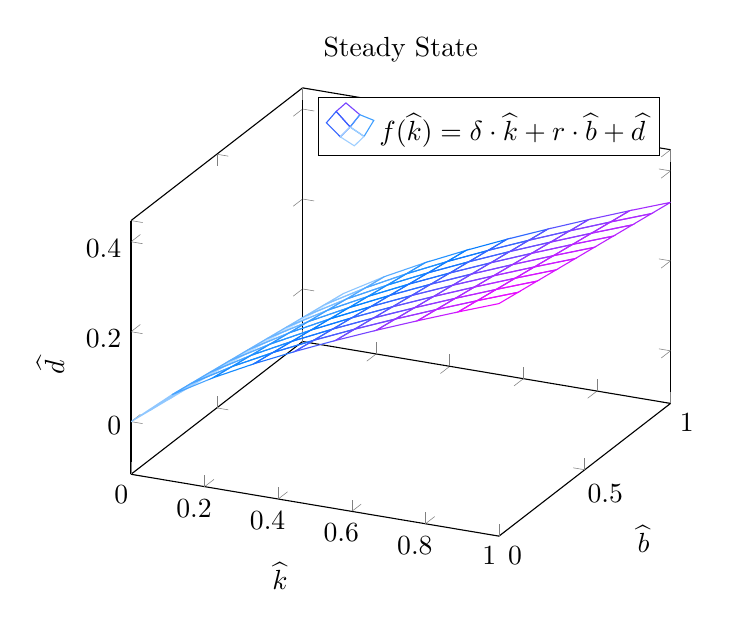
\begin{tikzpicture}
        \begin{axis}[
            title=Steady State,
            colormap/cool,
            xlabel= \(\widehat{k}\),
            ylabel= \(\widehat{b}\),
            zlabel=\(\widehat{d}\)
        ]
        \addplot3[
            mesh,
            samples=10,
            domain=0:1,
        ]
        {0.5*x^0.8-0.1*x-0.07*y};

        \addlegendentry{\(f(\widehat{k} ) = \delta \cdot \widehat{k} + r \cdot \widehat{b} + \widehat{d}\)}
        \end{axis}
    \end{tikzpicture}
    \caption{The three-dimensional plot delineates the steady state locus as defined by equation \ref{eq5'}, where the
    production function parameter values are set as \(\delta =0.1\), \(r=0.1\), \(\alpha=0.8\), and \(Z=0.5\). It
    highlights how at any steady-state level of capital \(\widehat{k}\), an increment in debt \(\widehat{b}\) necessitates a
    decline in dividends \(\widehat{d}\), illustrating the trade-off between debt servicing and dividend distribution.}


    \label{fig:steadystate3d}
\end{figure}

The figure illustrates the steady state relationships among debt (\(\widehat{b}\)), capital (\(\widehat{k}\)), and
dividends  (\(\widehat{d}\)) in a three-dimensional plot. The graph demonstrates how various combinations of debt and
capital influence the distribution of dividends. It is evident that, for any given level of \(\hat{k}\), a higher level of debt results in lower
dividends, as a larger portion of resources is allocated towards servicing interest payments. 
\vspace{1cm}